\documentclass[12pt]{article}
\usepackage{algorithm2e}
\usepackage{amsmath}
\usepackage{amssymb}
\usepackage{mathtools}
\usepackage{graphicx}
\usepackage{caption}
\usepackage{float}
\usepackage[utf8]{inputenc}
\usepackage{geometry}
\usepackage{multirow}
\usepackage{listings}
\usepackage{xcolor}
\usepackage{fancyvrb}
\usepackage{longtable}
\usepackage{polski}
\geometry{a4paper, margin=1in}

\title{Rozwiązanie Listy 2 z Metod Optymalizacji}
\author{Mikołaj Krupiński}

\begin{document}

\maketitle

\section*{Zadanie 1}

W pierwszym zadaniu należy zaplanować cięcia desek w tartaku produkującym deski o~ustalonej szerokości $W$ w calach według zapotrzebowania $d_1, d_2, \dots, d_k$ na deski o szerokościach $w_1, w_2 \dots, w_k$ w calach.

W tym celu wyznaczam wszytskie możliwości cięcia desek o szerokości $W$ na deski o~szerokościach $w_1, w_2 \dots, w_k$. Oznaczmy je jako $c_1, c_2, \dots, c_n$. Każde $c_i$ jest postaci $(i_1, i_2, \dots, i_k)$, gdzie $i_j$ jest liczbą naturalną oznaczającą ilość desek o szerokości $w_j$ w~cięciu $c_i$.

Celem zadania jest znalezienie harmonogramu produkcji minimalizaującego łączne odpadadki desek.

Zmiennymi decyzyjnymi w proponowanym modelu są
\begin{flalign*}
    && x_{i} \in \mathbb{N} && i \in \{1,\dots,n\}, &&
\end{flalign*}
gdzie $x_i$ oznacza liczbę desek ciętych w sposób $c_i$.

Jedyne ograniczenie zapewnia zaspokojenie zapotrzebowania na deski każdej szerokości.
\begin{flalign*}
    && \sum_{j=1}^{n} \left( x_j \cdot c_{i,j} \right) \geq d_i && \forall i \in \{1,\dots,k\} &&
\end{flalign*}

Funckją celu jest suma wyprodukowanych odpadków desek.
$$ W \cdot \left( \sum_{i=1}^{n} x_i \right) - \left( \sum_{i=0}^{k} w_i \cdot d_i \right) \to min $$

Dla danych podanych w treści zadania łączna ilość odpaków wynosi 18 cali, a cięcia deski wyglądają następująco.

\begin{table}[H]
    \centering
    \begin{tabular}{|c|c|c|c|c|}
        \hline
        Sposób cięcia & Ilość cięć \\ [0.5ex]
        \hline
        7 7 5 3 & 37 \\
        7 5 5 5 & 28 \\
        7 3 3 3 3 3 & 9 \\
        \hline
    \end{tabular}
    \caption{Cięcia desek}
\end{table}

Zwrócone rozwiązanie jest dopuszczalne.

\section*{Zadanie 2}

W drugim zadaniu dany jest zbiór zadań $J=\{1,\dots,n\}$, które muszą zostać wykonane na jednej maszynie. Dla każdego zadania $j \in J$ dany jest czas jego wykonania $p_j$, waga $w_j$ oraz moment $r_j$ przed, którym nie może ono być rozpoczęte. Celem jest znalezienie harmonogramu minimalizującego ważony czas zakończenia zadań, tj. $\sum_{j \in J} w_j \cdot C_j$, gdzie $C_j$ oznacza czas zakończenia zadania $j$.

Oznaczmy maksymalny możliwy czas zakończenia wszytskich zadań jako
$$T = \max_{j \in J}\{r_j\} + \sum_{j \in J}p_j + 1.$$
Wtedy zmiennymi decyzyjnymi są
\begin{flalign*}
    && x_{j,t} \in \{0,1\} && j \in J, t \in \{1,\dots,T\}, &&
\end{flalign*}
gdzie $x_{j,t} = 1$ oznacza, że zadanie $j$ rozpoczyna się w momencie $t$.

Każde zadanie $j$ powinno zostać wykonane dokładnie raz. Stąd poniższe ograniczenie.
\begin{flalign*}
    && \sum_{t=1}^{T} x_{j,t} = 1 && \forall j \in J &&
\end{flalign*}

Należy także zapewnić, że każde zadanie $j$ rozpocznie się najwcześniej w momencie $r_j$.
\begin{flalign*}
    && \sum_{t=0}^{r_j-1} x_{j,t} = 0 && \forall j \in J &&
\end{flalign*}

Ponadto zadania nie mogą być wykonywane równocześnie.
\begin{flalign*}
    && \sum_{j \in J} \left(\sum_{s=\max\{1,t+1-p_j\}}^{t} x_{j_s} \right) \leq 1 && \forall t \in \{1,\dots,T\} &&
\end{flalign*}

Funckją celu jest suma ważonych czasów zakończenia zadań.
$$ \sum_{j \in J} \sum_{t=1}^{T} \left( x_{j,t} \cdot w_j \cdot (t - 1 + p_j) \right) \to min $$

Użyłem modelu do rozwiązania zadania dla $n=10$ zadań o parametrach jak w tabeli poniżej.
\begin{table}[H]
    \centering
    \begin{tabular}{|c|c|c|c|}
        \hline
        Numer zadania & Czas wykonania & Waga & Moment rozpoczęcia \\ [0.5ex]
        \hline
        1 & 14 & 62 & 4 \\
        2 & 3 & 14 & 1 \\
        3 & 18 & 87 & 6 \\
        4 & 5 & 23 & 0 \\
        5 & 11 & 55 & 3 \\
        6 & 7 & 39 & 9 \\
        7 & 2 & 5 & 2 \\
        8 & 16 & 70 & 5 \\
        9 & 9 & 33 & 7 \\
        10& 4 &48&1\\
        \hline
    \end{tabular}
    \caption{Parametry zadań}
\end{table}

Optymalny harmonogram ma ważoną sumę czasów zakończenia równą 19681, a jego diagram przedstawia się jak na rysunku \ref{fig:ex2-diagram}.

\begin{figure}[H]
    \centering
    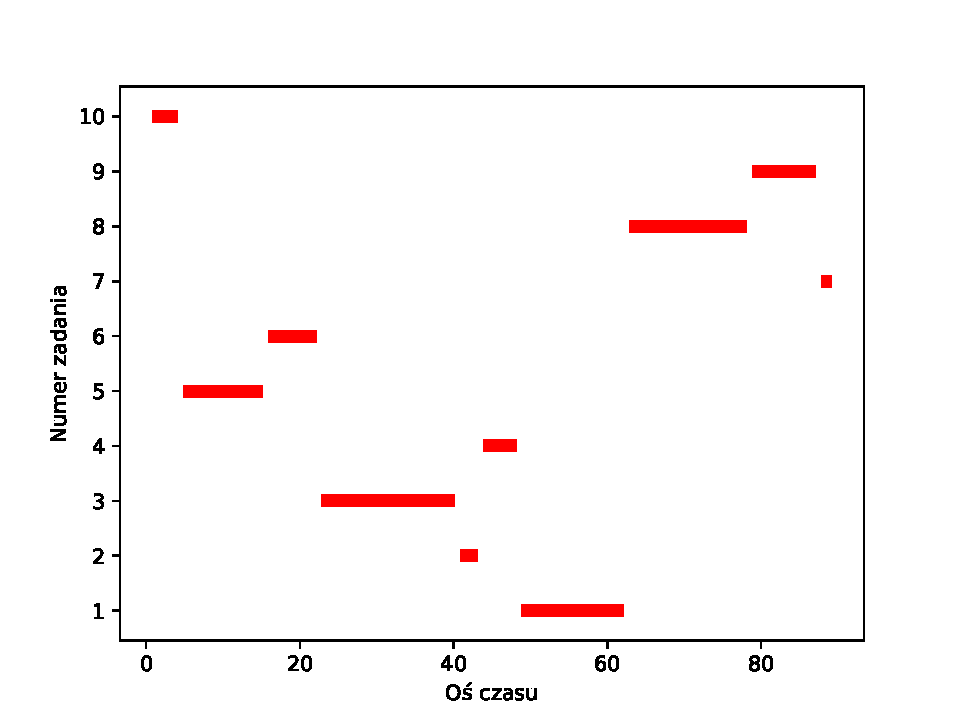
\includegraphics[width=0.8\textwidth]{ex2-diagram.pdf}
    \caption{Optymalny harmonogram wykonania zadań}
    \label{fig:ex2-diagram}
\end{figure}

Zwrócone rozwiązanie jest dopuszczalne.

\section*{Zadanie 3}

W trzecim zadaniu podobnie mamy zbiór zadań $J=\{1,\dots,n\}$, który musi zostać wykonany na $m$ maszynach. Dla każdego zadania $i$ dany jest czas jego wykonania $p_i$. Ponadto dany jest częściowy porządek $P$ na zbiorze zadań $J$ postaci $P=\{(i_1,i_2),\dots,(i_{k-1},i_k)\}$, który oznacza, że zadanie $i_1$ musi zostać wykonane przed rozpoczęciem zadania $i_2$ i podobnie dla pozostałych par. Celem jest znalezienie harmonogramy, który minimalizuje czas zakończenia wszytskich zadań. Oznaczmy go przez $C_{max}$.

Podobnie jak w poprzednim zadaniu Oznaczmy maksymalny możliwy czas zakończenia wszytskich zadań jako $T = \sum_{i \in J}p_i + 1$.

Zmiennymi decyzyjnymi w moim modelu są
\begin{flalign*}
    && x_{i,j,t} \in \{0,1\} && i \in J, j \in \{1,\dots,m\}, t \in \{1,\dots,T\}, &&
\end{flalign*}
gdzie $x_{i,j,t} = 1$ oznacza, że zadanie $i$ rozpoczyna się na maszynie $j$ w momencie $t$. Ponadto dodaję pomocniczą zmienną decyzyjną oznaczającą czas zakończenia ostatniego zadania.
$$ C_{max} \in \mathbb{N} $$

Pierwsze ograniczenie zapewnia, że $C_{max}$ ma wartość nie mniejszą niż czas zakończenia każdego z zadań.
\begin{flalign*}
    && C_{max} \geq x_{i,j,t}(t-1+p_i) && \forall i \in J, j \in \{1,\dots,m\}, t \in \{1,\dots,T\} &&
\end{flalign*}

Kolejne ograniczenie zapewnia, że każde zadanie zostanie wykonane dokładnie raz na jednej z maszyn.
\begin{flalign*}
    && \sum_{j=1}^{m} \sum_{t=1}^{T} x_{i,j,t} = 1 && \forall i \in J &&
\end{flalign*}

Zadania na jednej maszynie nie mogą być wykonywane równocześnie.
\begin{flalign*}
    && \sum_{i \in J} \left( \sum_{s=\max\{1,t+1-p_i\}}^{t} x_{i,j,s} \right) \leq 1 && \forall j \in \{1,\dots,m\}, t \in \{1,\dots,T\} &&
\end{flalign*}

Na koniec musimy zapewnić, że częściowy porządek $P$ jest spełniony, czyli każde zadanie wykonuje się po swoim poprzedniku.
\begin{flalign*}
    && \sum_{j=1}^{m} \sum_{t=1}^{T+1-p_i} x_{i,j,t} (t - 1 + p_i) \leq \sum_{j=1}^{m} \sum_{t=1}^{T+1-p_k} x_{k,j,t} (t - 1 + p_k) && \forall (i,k) \in P &&
\end{flalign*}

Funckją celu jest $C_{max}$, które minimalizujemy.
$$ C_{max} \to min $$

Dla danych z treści zadania $C_{max} = 9$, a harmonogram wygląda jak poniżej.

\begin{figure}[H]
    \centering
    \begin{BVerbatim}
M1: 3     699           
M2: 1 5888888           
M3: 2244777
    \end{BVerbatim}
\end{figure}

Zwrócone rozwiązanie jest dopuszczalne.

\section*{Zadanie 4}

W czwartym zadaniu musimy wykonać zbiór czynności $Z=\{1,\dots,n\}$ przy użyciu $p$ zasobów $R_1,\dots,R_p$. Dla każdego zasobu $R_i$ dany jest jego limit $N_i$. Dla każdej czynności $j$ znamy czas jej wykonania $p_j$ oraz wektor zasobów $\boldsymbol{r}_j=[r_1,\dots,r_p]$ potrzebnych do jego wykonania. Zbiór $Z$ jest częściowo uporządkowany przez relację $P$ postaci $P=\{(i_1,i_2),\dots,(i_{k-1},i_k)\}$, która oznacza, że czynność $i_1$ musi zostać wykonana przed rozpoczęciem czynności $i_2$ i podobnie dla pozostałych par. Celem jest znalezienie harmonogramu, który minimalizuje czas zakończenia wszytskich czynności.

Definiujemy maksymalny czas, po którym wszytskie zadania muszą zostać skończone jako $T=\sum_{j \in Z} p_j + 1$.

Zmiennymi decyzyjnymi w moim modelu są
\begin{flalign*}
    && x_{j,t} \in \{0,1\} && j \in Z, t \in \{1,\dots,T\}, &&
\end{flalign*}
gdzie $x_{j,t} = 1$ oznacza, że czynność $j$ rozpoczyna się w momencie $t$.

Definiujemy także pomocniczą zmienną decyzyjną oznaczającą czas zakończenia ostatniej czynności.
$$ C_{max} \in \mathbb{N} $$

Pierwsze ograniczenie zapewnia, że $C_{max}$ ma wartość nie mniejszą niż czas zakończenia każdej z czynności.
\begin{flalign*}
    && C_{max} \geq x_{j,t}(t-1+p_j) && \forall j \in Z, t \in \{1,\dots,T\} &&
\end{flalign*}

Kolejne ograniczenie gwarantuje, że każda czynność zostanie wykonana dokładnie raz.
\begin{flalign*}
    && \sum_{t=1}^{T} x_{j,t} = 1 && \forall j \in Z &&
\end{flalign*}

W żadnym momencie nie może zostać przekroczona podaż zasobów.
\begin{flalign*}
    && \sum_{j \in Z} \left( \sum_{s=\max\{1,t+1-p_j\}}^{t} x_{j,s} \cdot r_{j,i} \right) \leq N_i && \forall i \in \{1,\dots,p\}, t \in \{1,\dots,T\} &&
\end{flalign*}

Ostatnie ograniczenie zapewnia, że częściowy porządek $P$ jest spełniony, czyli każda czynność wykonuje się po swoim poprzedniku.
\begin{flalign*}
    && \sum_{t=1}^{T+1-p_i} x_{i,t} (t - 1 + p_i) \leq \sum_{t=1}^{T+1-p_j} x_{j,t} (t - 1) && \forall (i,j) \in P &&
\end{flalign*}

Funckją celu jest $C_{max}$, które minimalizujemy.
$$ C_{max} \to min $$

Dla danych przedtawionych w treści zadania $C_{max} = 237$, a harmonogram jak na rysunku \ref{fig:ex4-diagram}. Czerwonymi prostokątami oznaczone są kolejne czynności w czasie ich wykonywania, a niebieska krzywa oznacza ilość używanych zasobów w każdym momencie.

\begin{figure}[H]
    \centering
    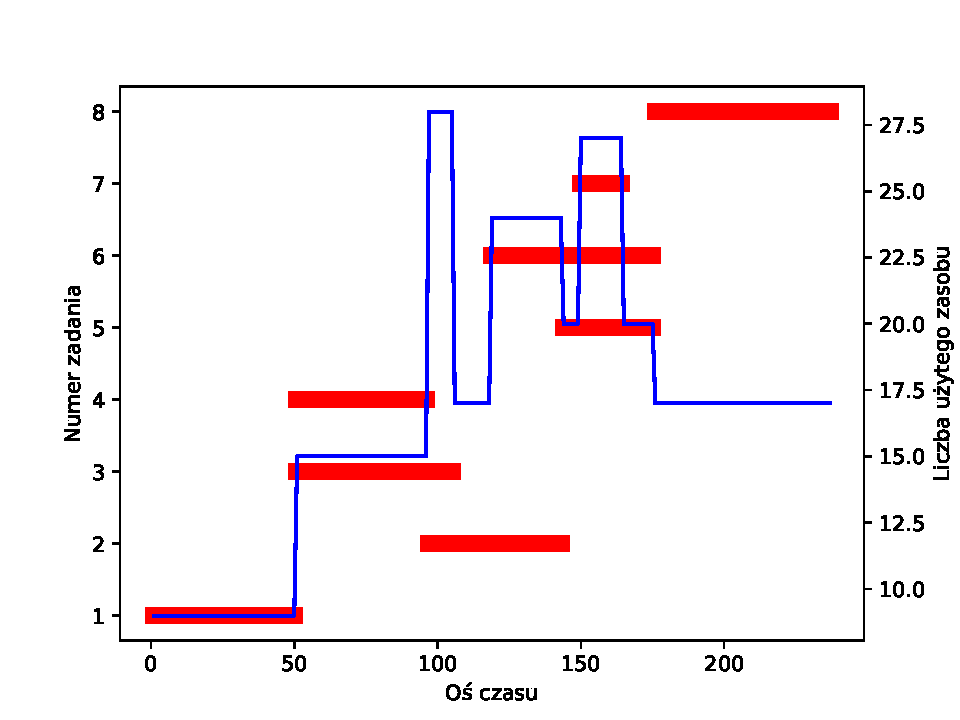
\includegraphics[width=0.8\textwidth]{ex4-diagram.pdf}
    \caption{Optymalny harmonogram wykonania czynności}
    \label{fig:ex4-diagram}
\end{figure}

Zwrócone rozwiązanie jest dopuszczalne.

\end{document}